%\documentclass[xcolor=table,handout,compress]{beamer}
\documentclass[xcolor=table]{beamer}
%--------------------------------------------------------------------------
% Common packages
%--------------------------------------------------------------------------
\usepackage[english]{babel}
\usepackage{pgfpages} % required for notes on second screen
\usepackage{graphicx}
\usepackage{subfigure}
\usepackage{multicol}
\usepackage[normalem]{ulem}

\usepackage{tabularx,ragged2e}
\usepackage{booktabs}
\usepackage{marvosym}

\makeatletter
\let\beamer@writeslidentry@miniframeson=\beamer@writeslidentry
\def\beamer@writeslidentry@miniframesoff{%
  \expandafter\beamer@ifempty\expandafter{\beamer@framestartpage}{}% does not happen normally
  {%else
    % removed \addtocontents commands
    \clearpage\beamer@notesactions%
  }
}
\newcommand*{\miniframeson}{\let\beamer@writeslidentry=\beamer@writeslidentry@miniframeson}
\newcommand*{\miniframesoff}{\let\beamer@writeslidentry=\beamer@writeslidentry@miniframesoff}
\makeatother


%--------------------------------------------------------------------------
% Load theme
%--------------------------------------------------------------------------
\usetheme{hri}

\usepackage{tikz}
\usetikzlibrary{patterns,shapes,fpu,fit,calc,mindmap,backgrounds,positioning,svg.path}

\tikzset{
  invisible/.style={opacity=0},
  visible on/.style={alt={#1{}{invisible}}},
  alt/.code args={<#1>#2#3}{%
    \alt<#1>{\pgfkeysalso{#2}}{\pgfkeysalso{#3}} % \pgfkeysalso doesn't change the path
  },
}

\newcommand*\circled[1]{\tikz[baseline=(char.base)]{
            \node[shape=circle,draw,inner sep=1pt] (char) {\bf\tiny #1};}}


%% Neat trick to have only one navigation bullet per subsection
%% http://tex.stackexchange.com/questions/64333/one-navigation-bullet-per-subsection-with-subsection-false-in-custom-beamer-them
%\usepackage{etoolbox}
%\makeatletter
%\patchcmd{\slideentry}{\advance\beamer@xpos by1\relax}{}{}{}
%\def\beamer@subsectionentry#1#2#3#4#5{\advance\beamer@xpos by1\relax}%
%\makeatother
%%%%%%%%%%%%%%%%%%%%%%%%%%%%%%%%%%%%%%%

\graphicspath{{figs/}}

% for model of anthopomorphism
\newcommand{\IPA}{{$\mathcal{A}_0$~}}
\newcommand{\SLA}{{$\mathcal{A}_\infty$~}}
\newcommand{\sla}{{\mathcal{A}_\infty}}
\newcommand{\AntMax}{{$\mathcal{A}_{max}$~}}
\newcommand{\antMax}{{\mathcal{A}_{max}}}

% for HATP plans
\newcommand{\hatpaction}[3]{#1\\\textsf{\scriptsize #2,}\\\textsf{\scriptsize #3}}
\newcommand{\stmt}[1]{{\footnotesize \tt  #1}}

% for mutual modelling
\newcommand{\Mmodel}[3]{{\mathcal{M}(#1, #2, #3)}}
\newcommand{\model}[3]{{$\mathcal{M}(#1, #2, #3)$}}
\newcommand{\Model}[3]{{$\mathcal{M}^{\circ}(#1, #2, #3)$}}

% typeset logical concept
\newcommand{\concept}[1]{{\scriptsize \texttt{#1}}}

\newcommand{\backbutton}{\hfill\hyperlink{appendix}{\beamerreturnbutton{Supplementary material}}}
%--------------------------------------------------------------------------
% General presentation settings
%--------------------------------------------------------------------------
\title{\Large ROS for Human-Robot Interaction}
\subtitle{Towards REP-155}
\date{{\bf ROSCon} | Oct 2022}
\author{Séverin Lemaignan}
\institute{{\bf PAL Robotics} Senior Scientist AI \& Social Interactions}

%--------------------------------------------------------------------------
% Notes settings
%--------------------------------------------------------------------------
%\setbeameroption{show notes on second screen}
%\setbeameroption{hide notes}

\begin{document}


%%%%%%%%%%%%%%%%%%%%%%%%%%%%%%%%%%%%%%%%%%%%%%%%%%%%%%%%


%%%%%%%%%%%%%%%%%%%%%%%%%%%%%%%%%%%%%%%%%%%%%%%%%%%%%%%%

\licenseframe{github.com/severin-lemaignan/presentation-ros4hri}

\maketitle
\imageframe{my_background/00}


%\begin{frame}[plain]{}
%
%    \Large
%    \center
%    {\bf ROS REP-155 aka ROS4HRI}
%
%    \vspace{1em}
%    {\bf \href{https://www.ros.org/reps/rep-0155.html}{www.ros.org/reps/rep-0155.html}}
%
%    Still an ``\emph{open REP}'': will evolve based on community feedback (eg,
%    \textbf{you!})\\
%
%\end{frame}

{
    \paper{Mohamed, Lemaignan, \textbf{ROS for Human-Robot Interaction}, IROS 2021}
\begin{frame}{Why ROS4HRI?}

    \begin{itemize}
        \item  dealing with humans is actually hard: they keep on disappearing/reappearing; hard to predict where/when; ‘shape’ known at run-time only, etc.

\item widely different requirements depending on application: from ‘2D points’ to full online kinematic model.

    \item no ROS standard for HRI (nothing, nada, rien!)
    \end{itemize}

\end{frame}
}

{
    \paper{Mohamed, Lemaignan, \textbf{ROS for Human-Robot Interaction}, IROS 2021}
\begin{frame}{Design requirements}

    \begin{itemize}
        \item<1-> representations \textbf{application-agnostic}: from point-like crowd
            simulation, to kineastetic teaching, to social interaction
        \item<2-> does not enforce any specific algorithm or perception pipeline
        \item<3-> however, takes into account what current algorithms can or can not
            do {\footnotesize (eg: kinematic model of human)}
        \item<4-> integrated as much as possible with existing ROS conventions
            {\footnotesize (eg: \texttt{robot\_state\_publisher} for human forward
            kinematics)}
    \end{itemize}
\end{frame}

\begin{frame}{Scope}
    \begin{itemize}
        \item<+-> set of new messages (\texttt{hri\_msgs})
        \item<+-> topics naming convention
        \item<+-> \texttt{tf} frames naming convention
        \item<+-> (parametric) kinematic model of humans
        \item<+-> (a few) global ROS parameters
    \end{itemize}

    \begin{itemize}
        \item<+-> for now, focus on \emph{perception} only
        \item<+-> initially, ROS1
    \end{itemize}
\end{frame}
}

\begin{frame}{Human representation: permanent vs transient IDs}

        \includegraphics<1>[width=0.9\linewidth]{ros4hri/ids_0}
        \includegraphics<2>[width=0.9\linewidth]{ros4hri/ids_1}
        \includegraphics<3>[width=0.9\linewidth]{ros4hri/ids_2}
        \includegraphics<4>[width=0.9\linewidth]{ros4hri/ids_3}
        \includegraphics<5>[width=0.9\linewidth]{ros4hri/ids_4}
        \includegraphics<6>[width=0.9\linewidth]{ros4hri/ids_5}
\end{frame}

%\begin{frame}{Semantic of IDs}
%    \scriptsize
%    \begin{tabular}{@{}lllp{6.5cm}@{}}
%\toprule
%\textbf{Face ID} & \textbf{Body ID} & \textbf{Person ID} & \textbf{Interpretation}                                                                                                                                                                                                                                                                 \\ \midrule
%        \texttt{\#24ac }          & \texttt{Ø     }           & \texttt{Ø     }             & \tiny Face detected - random id \texttt{\#24ac} assigned - corresponding TF frame \texttt{/face\_24ac} is published.                                                                                                                                                                                            \\
%        \texttt{\#d73b }          & \texttt{Ø     }           & \texttt{Ø     }             & \tiny Face detected (possibly a re-detection of a previous one) - random id \texttt{\#d73b} assigned + frame published.                                                                                                                                                                                \\
%        \texttt{Ø      }          & \texttt{\#37ef}           & \texttt{Ø     }             & \tiny Skeleton detected - id \texttt{\#37ef} assigned + frame \texttt{/body\_37ef} published.                                                                                                                                                                                                                   \\
%        \texttt{\#d73b }          & \texttt{\#37ef}           & \texttt{Ø     }             & \tiny Face/body matcher merged the face and the skeleton into a single agent. The 2 previous records do not exist any more independently.                                                                                                                                                     \\
%        \texttt{Ø      }          & \texttt{Ø     }           & \texttt{\#9d8a}             & \tiny Human \texttt{\#9d8a} is known, but not associated to any face or body. Note that TF frame \texttt{/person\_9d8a} might nevertheless exist (for instance, last known position of the human).                                                                                                              \\
%        \texttt{\#d73b }          & \texttt{Ø     }           & \texttt{\#9d8a}             & \tiny Face \texttt{\#d73b} is associated to human \texttt{\#9d8a}. Typical result of successful face recognition.                                                                                                                                                                                               \\
%        \texttt{\#96f1 }          & \texttt{Ø     }           & \texttt{\#9d8a}             & \tiny Human \texttt{\#9d8a} is now associated to face \texttt{\#96f1}: this new association might come from the face tracker losing track of a previous face, thus re-assigning a different id to the face. The newly assigned face is however recognized by the face recognition module as being human \texttt{\#9d8a}. \\
%        \texttt{\#96f1 }          & \texttt{\#37ef}           & \texttt{\#9d8a}             & \tiny The human \texttt{\#9d8a} is fully tracked: both the head and the body are detected.                                                                                                                                                                                                             \\
%        \texttt{Ø      }          & \texttt{\#37ef}           & \texttt{\#9d8a}             & \tiny Only the body of human \texttt{\#9d8a} is tracked: this situation typically occurs if the face trackers loses the face after facial recognition successfully identified the human, and while the skeleton tracker still tracks the body.                                                         \\
%        \texttt{Ø      }          & \texttt{Ø     }           & \texttt{\#b3da}             & \tiny \texttt{\#b3da} is another human, considered by the robot as different to \texttt{\#9d8a}.                                                                                                                                                                                                      \\ \bottomrule
%\end{tabular}
%\end{frame}

\begin{frame}{Topics structure: faces}

    Under \textbf{\texttt{/humans/faces/<faceID>/}} (eg \texttt{/humans/faces/bf3d}):

    \scriptsize
    \begin{tabular}{@{}llp{4cm}@{}}
        \toprule
\textbf{Name} & \textbf{Message type}         & \textbf{Description}                                                \\ \midrule
        \texttt{/roi       }   & \texttt{hri\_msgs/NormalizedRegi...} & Region of the face in the source image                              \\
        \texttt{/cropped       }   & \texttt{sensor\_msgs/Image} & Cropped face                              \\
        \texttt{/frontalized       }   & \texttt{sensor\_msgs/Image} & Frontalised face                              \\
        \texttt{/landmarks }   & \texttt{hri\_msgs/FacialLandmarks    } & The 2D facial landmarks extracted from the face                     \\
        \texttt{/facs      }   & \texttt{hri\_msgs/FacialActionUnits  } & The presence and intensity of facial action units found in the face \\
        \texttt{/expression}   & \texttt{hri\_msgs/Expression         } & The expression recognised from the face           \\
        \texttt{/softbiometrics      } & \texttt{hri\_msgs/SoftBiometrics }  &   Soft biometrics like age and gender of the face                                       \\  \bottomrule               
\end{tabular}
    
\end{frame}

\begin{frame}{Topics structure: bodies}

    Under \textbf{\texttt{/humans/bodies/<bodyID>/}} (eg \texttt{/humans/bodies/5e4d}):

    \scriptsize
    \begin{tabular}{@{}llp{4cm}@{}}
        \toprule
        \textbf{Name} & \textbf{Message type}         & \textbf{Description}                                                \\ \midrule
        \texttt{/roi       }   & \texttt{hri\_msgs/NormalizedRegi...} & Region of the whole body in the source image                              \\
        \texttt{/cropped       }   & \texttt{sensor\_msgs/Image} & Cropped image of the body                              \\
        \texttt{/joint\_states       }   & \texttt{sensor\_msgs/JointState} & The joint state of the human body                              \\
        \texttt{/skeleton2d}   & \texttt{hri\_msgs/Skeleton2D}        & The 2D points of the detected skeleton                              \\
        \texttt{/posture}    & \texttt{hri\_msgs/BodyPosture}      & Recognised body posture (sitting, standing)                                 \\
        \texttt{/gesture}    & \texttt{hri\_msgs/Gesture}      & Recognised symbolic gesture                                 \\
        \bottomrule               
\end{tabular}

    \vspace{1em}
    \emph{3D pose? \texttt{tf} frames from joint state + human URDF! I'll come to it
    in a minute.}
    
\end{frame}

\begin{frame}{Topics structure: voices}

    Under \textbf{\texttt{/humans/voices/<voiceID>/}} (eg~\texttt{/humans/voices/dde2}):

    \scriptsize
    \begin{tabular}{@{}llp{4cm}@{}}
        \toprule
        \textbf{Name} & \textbf{Message type}         & \textbf{Description}                                                \\ \midrule
        \texttt{/audio       } & \texttt{audio\_common\_msgs/AudioData  } & Separated audio stream for this voice                     \\
        \texttt{/features    } & \texttt{hri\_msgs/AudioFeatures} & INTERSPEECH’09 Emotion challenge low-level audio features \\
        \texttt{/is\_speaking} & \texttt{std\_msgs/Bool         } & Whether or not speech is recognised from this voice       \\
        \texttt{/speech      } & \texttt{hri\_msgs/LiveSpeech       } & The live stream of speech recognized via an ASR engine \\
        \bottomrule               
\end{tabular}
    
\end{frame}

\begin{frame}{Topics structure: persons}

    Under \textbf{\texttt{/humans/persons/<personID>/}} (eg~\texttt{/humans/persons/45ff}):

    \scriptsize
    \begin{tabular}{@{}llp{4cm}@{}}
        \toprule
        \textbf{Name} & \textbf{Message type}         & \textbf{Description}                                                \\ \midrule
        \texttt{/face\_id            } & \texttt{std\_msgs/String} (latched) & Face matched to that person (if any)                                                    \\
        \texttt{/body\_id            } & \texttt{std\_msgs/String} (latched) & Body matched to that person (if any)                                                    \\
        \texttt{/voice\_id           } & \texttt{std\_msgs/String} (latched) & Voice matched to that person (if any)                                                   \\
        \texttt{/alias           } & \texttt{std\_msgs/String} (latched) & ID of other person, if alias                                                    \\
        \texttt{/anonymous           } & \texttt{std\_msgs/Bool} (latched) & if true, anonymous person (not permanent ID)   \\
        \texttt{/engagement\_status} & \texttt{hri\_msgs/EngagementLevel        }  & engagement status of the person \emph{with the robot} \\
        \texttt{/location\_confidence} & \texttt{std\_msgs/Float32        }  & Location confidence; 1 means 'person currently seen', 0 means 'person location unknown' \\
        \texttt{/name                } & \texttt{std\_msgs/String         }  & Name, if known                                                                          \\
        \texttt{/native\_language    } & \texttt{std\_msgs/String         }  & IETF language codes like \texttt{EN\_gb}, if known    \\
\bottomrule
\end{tabular}
    
\end{frame}

\begin{frame}{Topics structure: groups}

    Under \textbf{\texttt{/humans/groups/<groupID>/}} (eg~\texttt{/humans/groups/56ef2}):

    \scriptsize
    \begin{tabular}{@{}llp{4cm}@{}}
        \toprule
        \textbf{Name} & \textbf{Message type}         & \textbf{Description}                                                \\ \midrule
        \texttt{/members                } & \texttt{hri\_msgs/IdLists         }  & Person ID of the members of the group  \\
\bottomrule
\end{tabular}

    \vspace{1em}\textbf{Attention:} not yet in the REP-155!
    
\end{frame}

\begin{frame}{Topics structure: interactions}

    Under \textbf{\texttt{/humans/interactions/}}:

    \scriptsize
    \begin{tabular}{@{}llp{4cm}@{}}
        \toprule
        \textbf{Name} & \textbf{Message type}         & \textbf{Description}                                                \\ \midrule
        \texttt{/gaze    } & \texttt{hri\_msgs/Gaze         }  & estimated gazing behaviours    \\
\bottomrule
\end{tabular}
    
\end{frame}

\begin{frame}{Human physical representation}

    \begin{columns}
        \begin{column}{0.4\linewidth}
            \begin{itemize}
                \item standard ROS pipeline: joint state (eg OpenPose, mediapipe) -> \texttt{robot\_state\_publisher} + URDF

                \item URDF generated on the fly, based on person’s height (xacro params)

                \item Follows REP-120 as much as possible.
            \end{itemize}
        \end{column}
        \begin{column}{0.6\linewidth}
            \begin{center}
                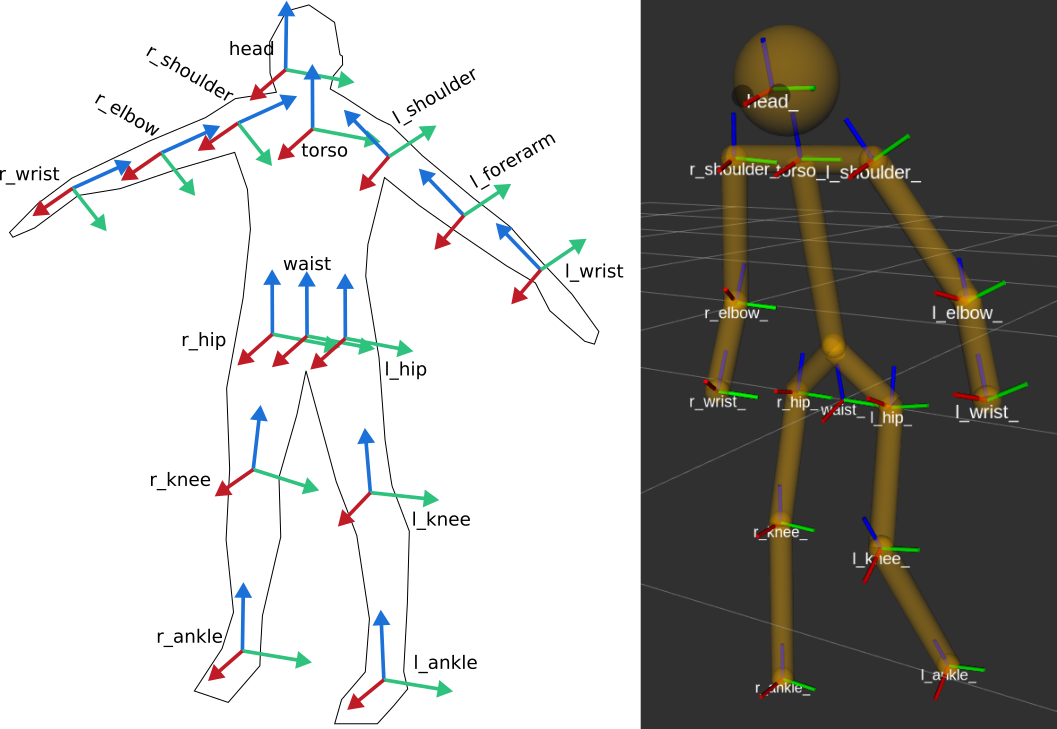
\includegraphics[width=\linewidth]{ros4hri/skeletons}
            \end{center}
        \end{column}
    \end{columns}
\end{frame}

\begin{frame}{Tooling}


    \begin{center}
    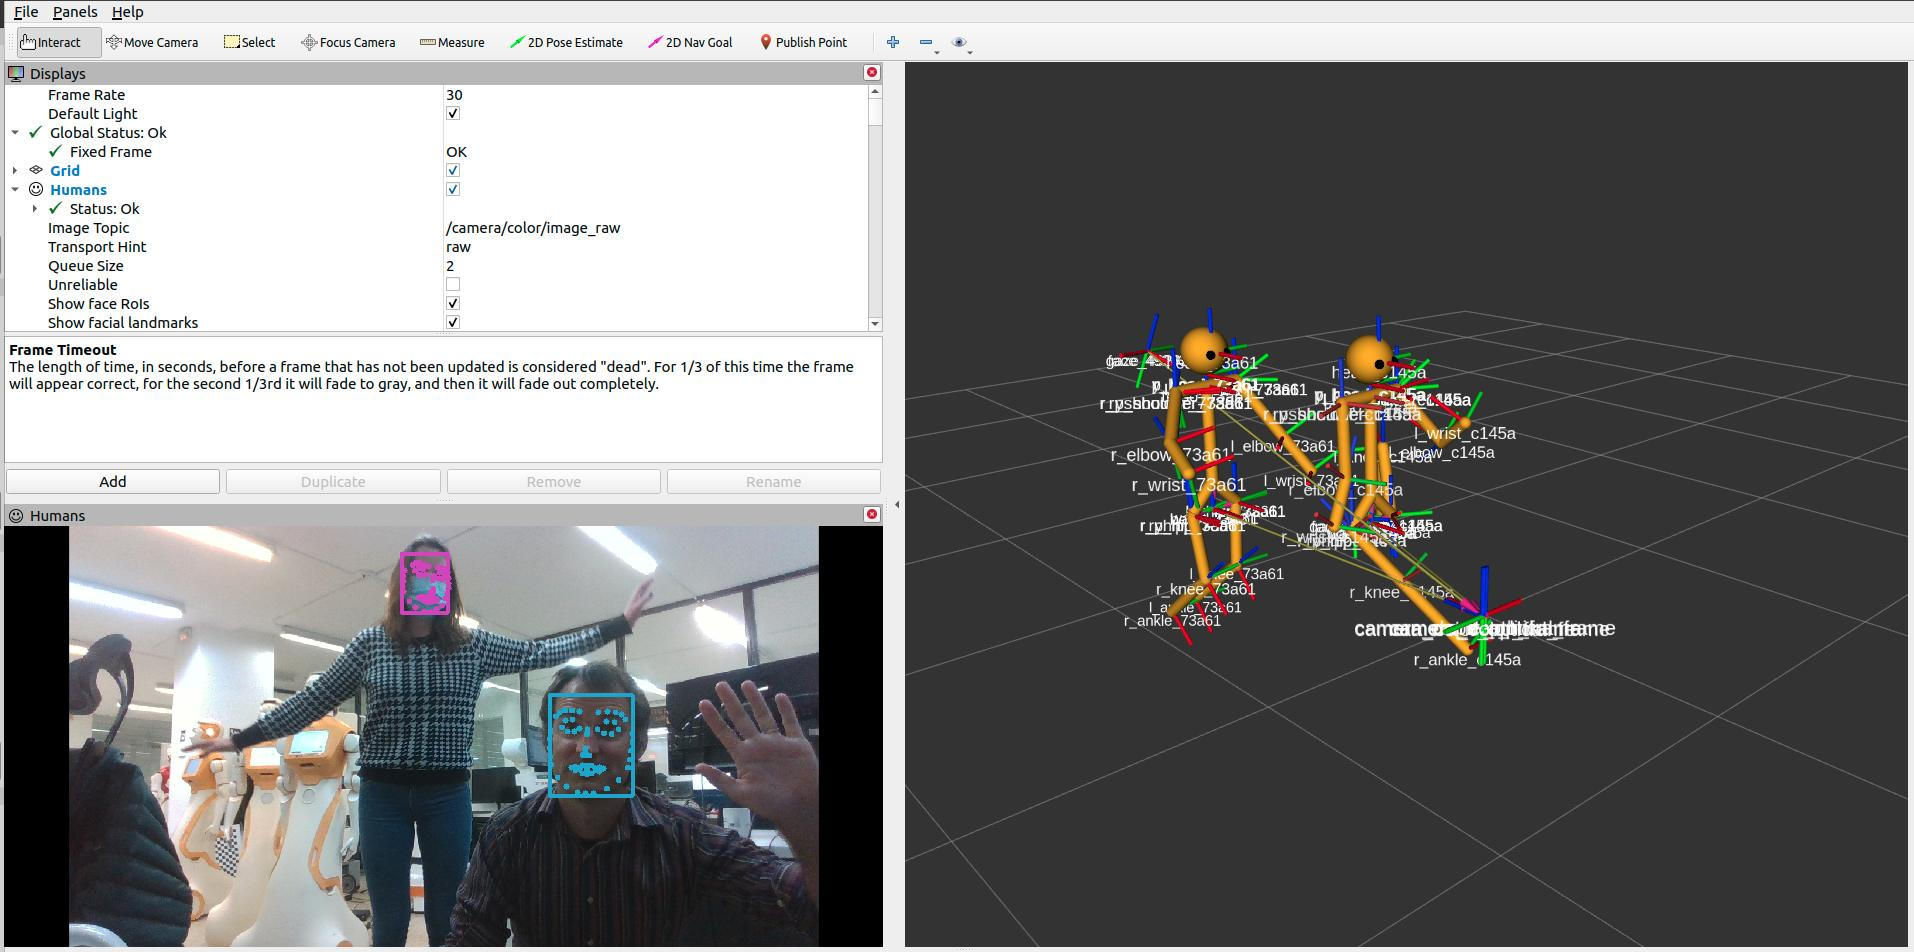
\includegraphics[width=8cm]{ros4hri/screenshot.jpg}
    \end{center}

    \vspace{1em}

    \begin{columns}
        \begin{column}{0.5\linewidth}
    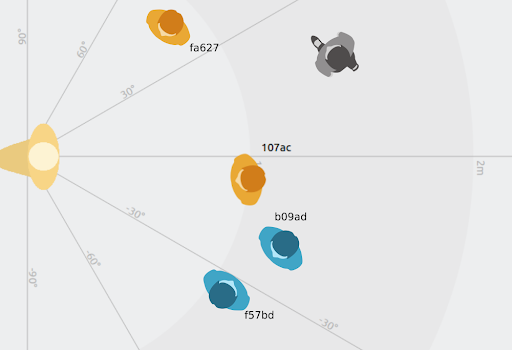
\includegraphics[width=0.8\linewidth]{ros4hri/rqt_humans.png}
        \end{column}
        \begin{column}{0.5\linewidth}
    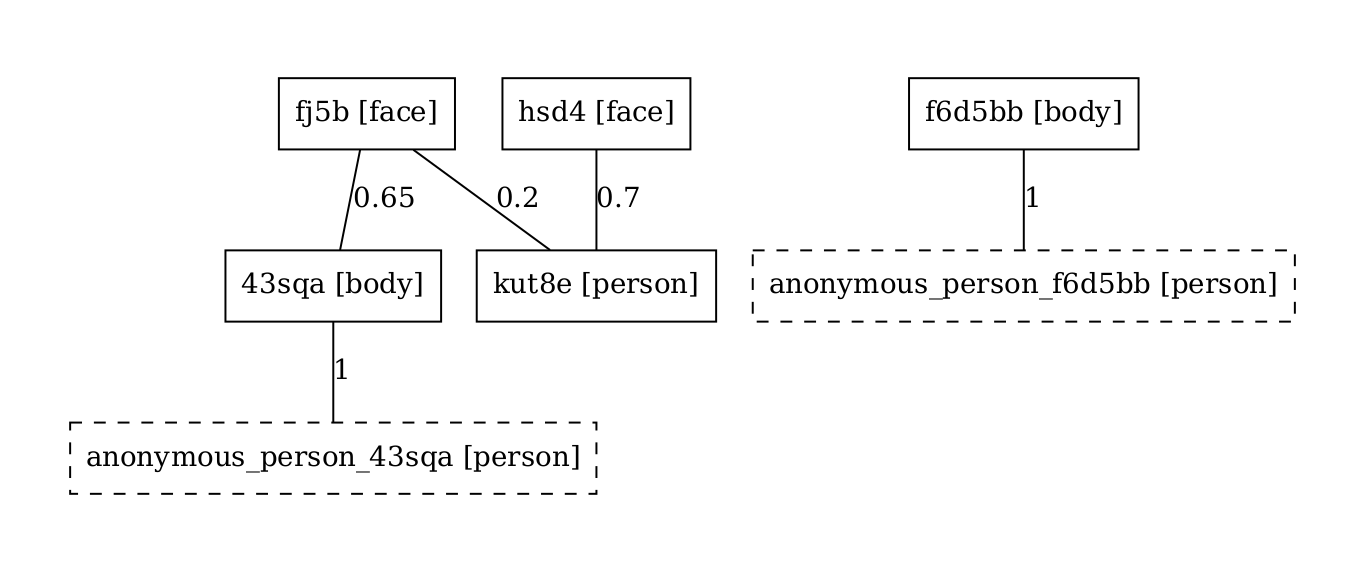
\includegraphics[width=6cm]{ros4hri/human_graph.png}
        \end{column}
    \end{columns}
\end{frame}





\begin{frame}{One possible pipeline (but other are possible!)}
    \begin{center}
        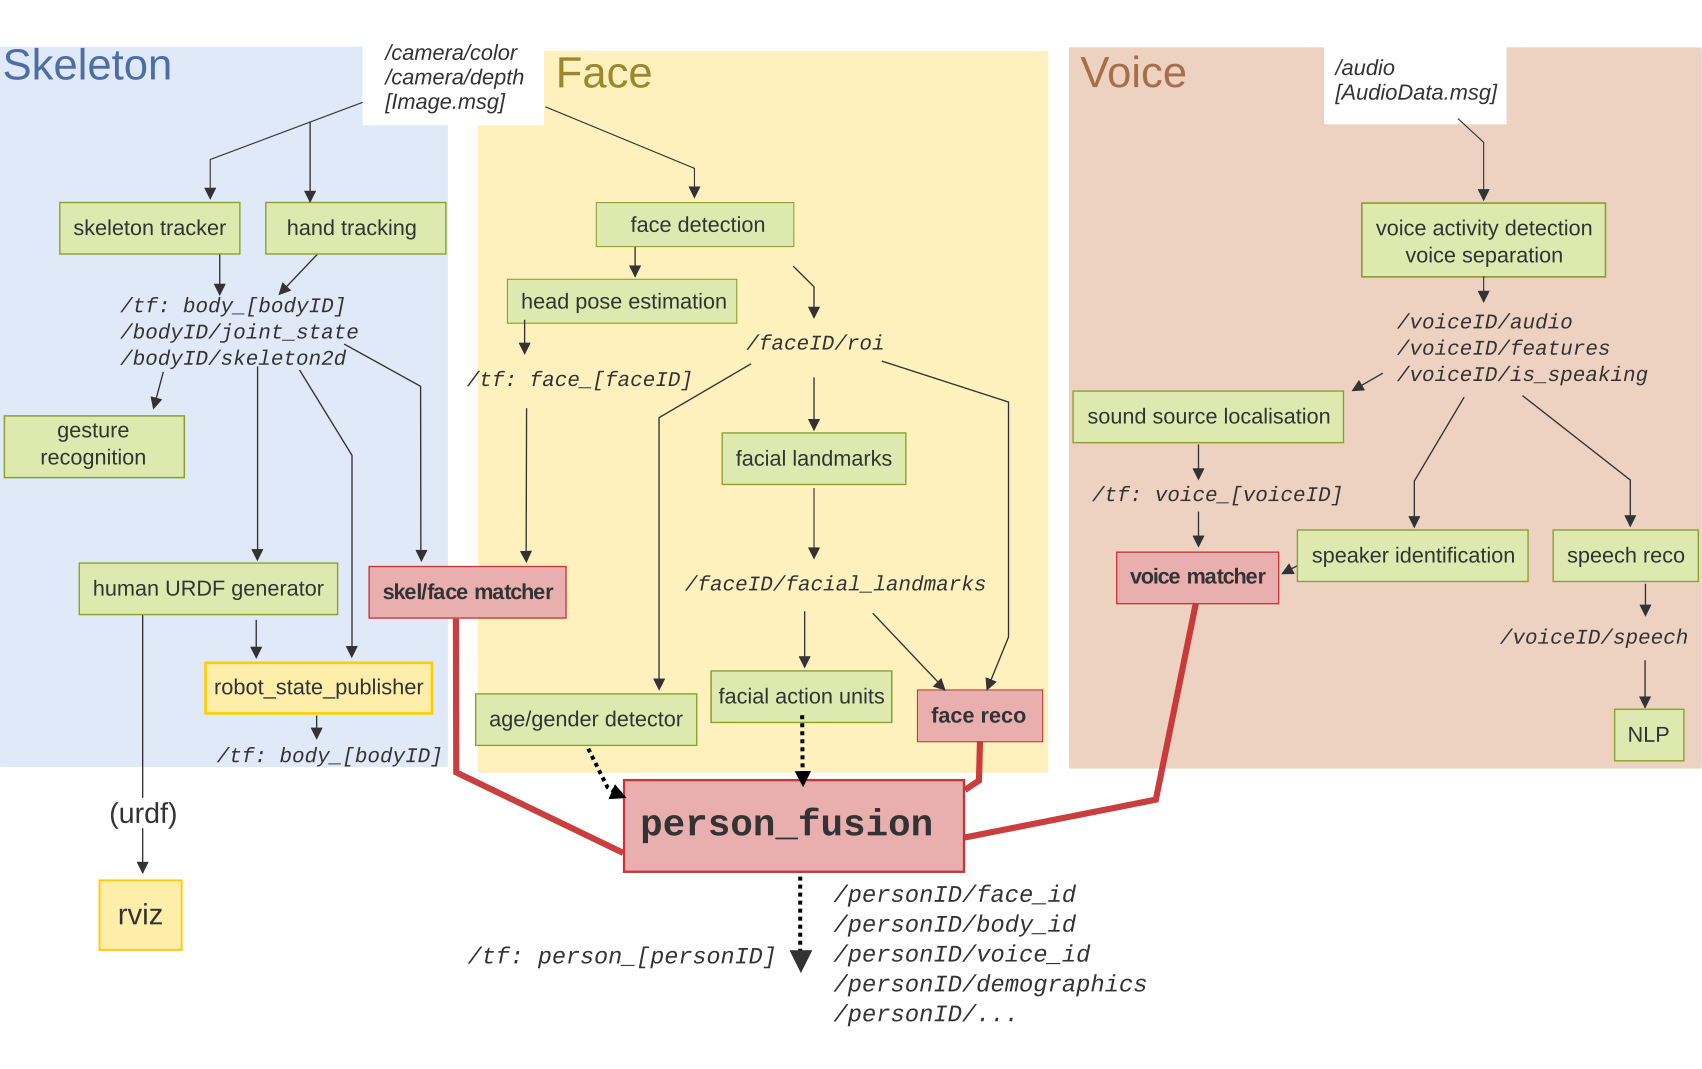
\includegraphics[height=7cm]{ros4hri/ros4hri-pipeline2}
    \end{center}
\end{frame}


\imageframe[scale=0.95]{ros4hri/ros4hri-status.png}



%%%%%%%%%%%%%%%%%%%%%%%%%%%%%%%%%%%%%%%%%%%%%%%%%%%%%%%%
{
    \fullbackground[color=black]{lastpage}
    \begin{frame}[plain]

        \begin{columns}
            \begin{column}{0.5\linewidth}
            \end{column}
            \begin{column}{0.5\linewidth}

                \setbeamercolor{hriSec1Demo}{fg=white!70!black}
                \vspace{14em}
                \begin{beamercolorbox}[wd=\linewidth,ht=6ex,dp=0.7ex]{hriSec1Demo}
                    \textbf{Thank you!}

                    \vspace{4em}

                    \footnotesize
                    Slides:\\
                    {\footnotesize\href{https://github.com/severin-lemaignan/presentation-ros4hri}{github.com/severin-lemaignan/presentation-ros4hri}}

                    \vspace{2em}

                    (btw, we are always looking for great people to join us: drop me line if you want to know more!)

                \end{beamercolorbox}
            \end{column}
        \end{columns}
    \end{frame}
}

\appendix
\imageframe[scale=0.9]{pd_comparison}

\end{document}
